% ==============================================================================
% Section 4.4: Temporal Dynamics (RQ3)
% ==============================================================================
\subsection{Temporal Dynamics (RQ3)}
\label{sec:temporal}

Having established that the four statuses cluster in different places, we now examine how those spatial patterns have evolved since 2015.
Table~\ref{tab:slopes} reports OLS trend slopes (Newey-West HAC standard errors, bandwidth = 12) for HH municipality counts by region and status.
Three regional narratives deserve attention.

\begin{tabular}{lrrrr}
  \toprule
  \textbf{Region} & \textbf{Total} & \textbf{Not Located} & \textbf{Located Alive} & \textbf{Located Dead} \\
  \midrule
  Norte & +0.55*** & +0.19 & +0.95*** & +0.54*** \\
  Norte-Occidente & +0.60*** & +0.44*** & +0.68*** & +0.06 \\
  Centro-Norte & -0.73*** & -0.50*** & -0.03 & +0.01 \\
  Centro & +2.82*** & +4.17*** & +3.13*** & +1.02*** \\
  Sur & +0.05 & +0.29*** & +0.12 & +0.03 \\
  Bajío & -0.99*** & +0.17 & -0.41* & +0.22* \\
  \bottomrule
  \multicolumn{5}{l}{\footnotesize OLS slope (municipalities per year $= $ slope $\times 12$), 132 monthly observations.} \\
  \multicolumn{5}{l}{\footnotesize $^{***}p<0.001$, $^{**}p<0.01$, $^{*}p<0.05$. Sign: positive $=$ growing hotspot region.} \\
\end{tabular}

\subsubsection{The Centro Expansion}

Centro emerges as the fastest-growing hotspot region across all four statuses---a finding that was invisible to prior annual analyses focused on the Norte--Baj\'{i}o axis.
Not Located HH municipalities in Centro grew at $+4.96$ municipalities per year ($p < 0.001$), the largest slope in the entire matrix.
Total ($+3.43$, $p < 0.001$), Located Alive ($+3.63$, $p < 0.001$), and Located Dead ($+1.26$, $p < 0.001$) all show significant positive trends.

Figure~\ref{fig:hh_trend} illustrates the divergent trajectories of Centro, Norte, and Baj\'{i}o.
The Centro expansion is visible as a steep upward trajectory beginning around 2019 for Not Located and accelerating through 2025.
This finding requires careful interpretation.
Two non-exclusive hypotheses may explain the pattern: (i) a real increase in disappearances in the metropolitan corridor spanning Estado de M\'{e}xico, CDMX, Puebla, Morelos, and Hidalgo---possibly reflecting urbanization of organized criminal violence; or (ii) a reporting artefact, whereby urban areas with more prosecutors, civil society organizations, and media attention register a higher proportion of disappearances even if underlying incidence did not increase as sharply.
We cannot distinguish between these hypotheses with RNPDNO data alone.

\begin{figure}[htbp]
  \centering
  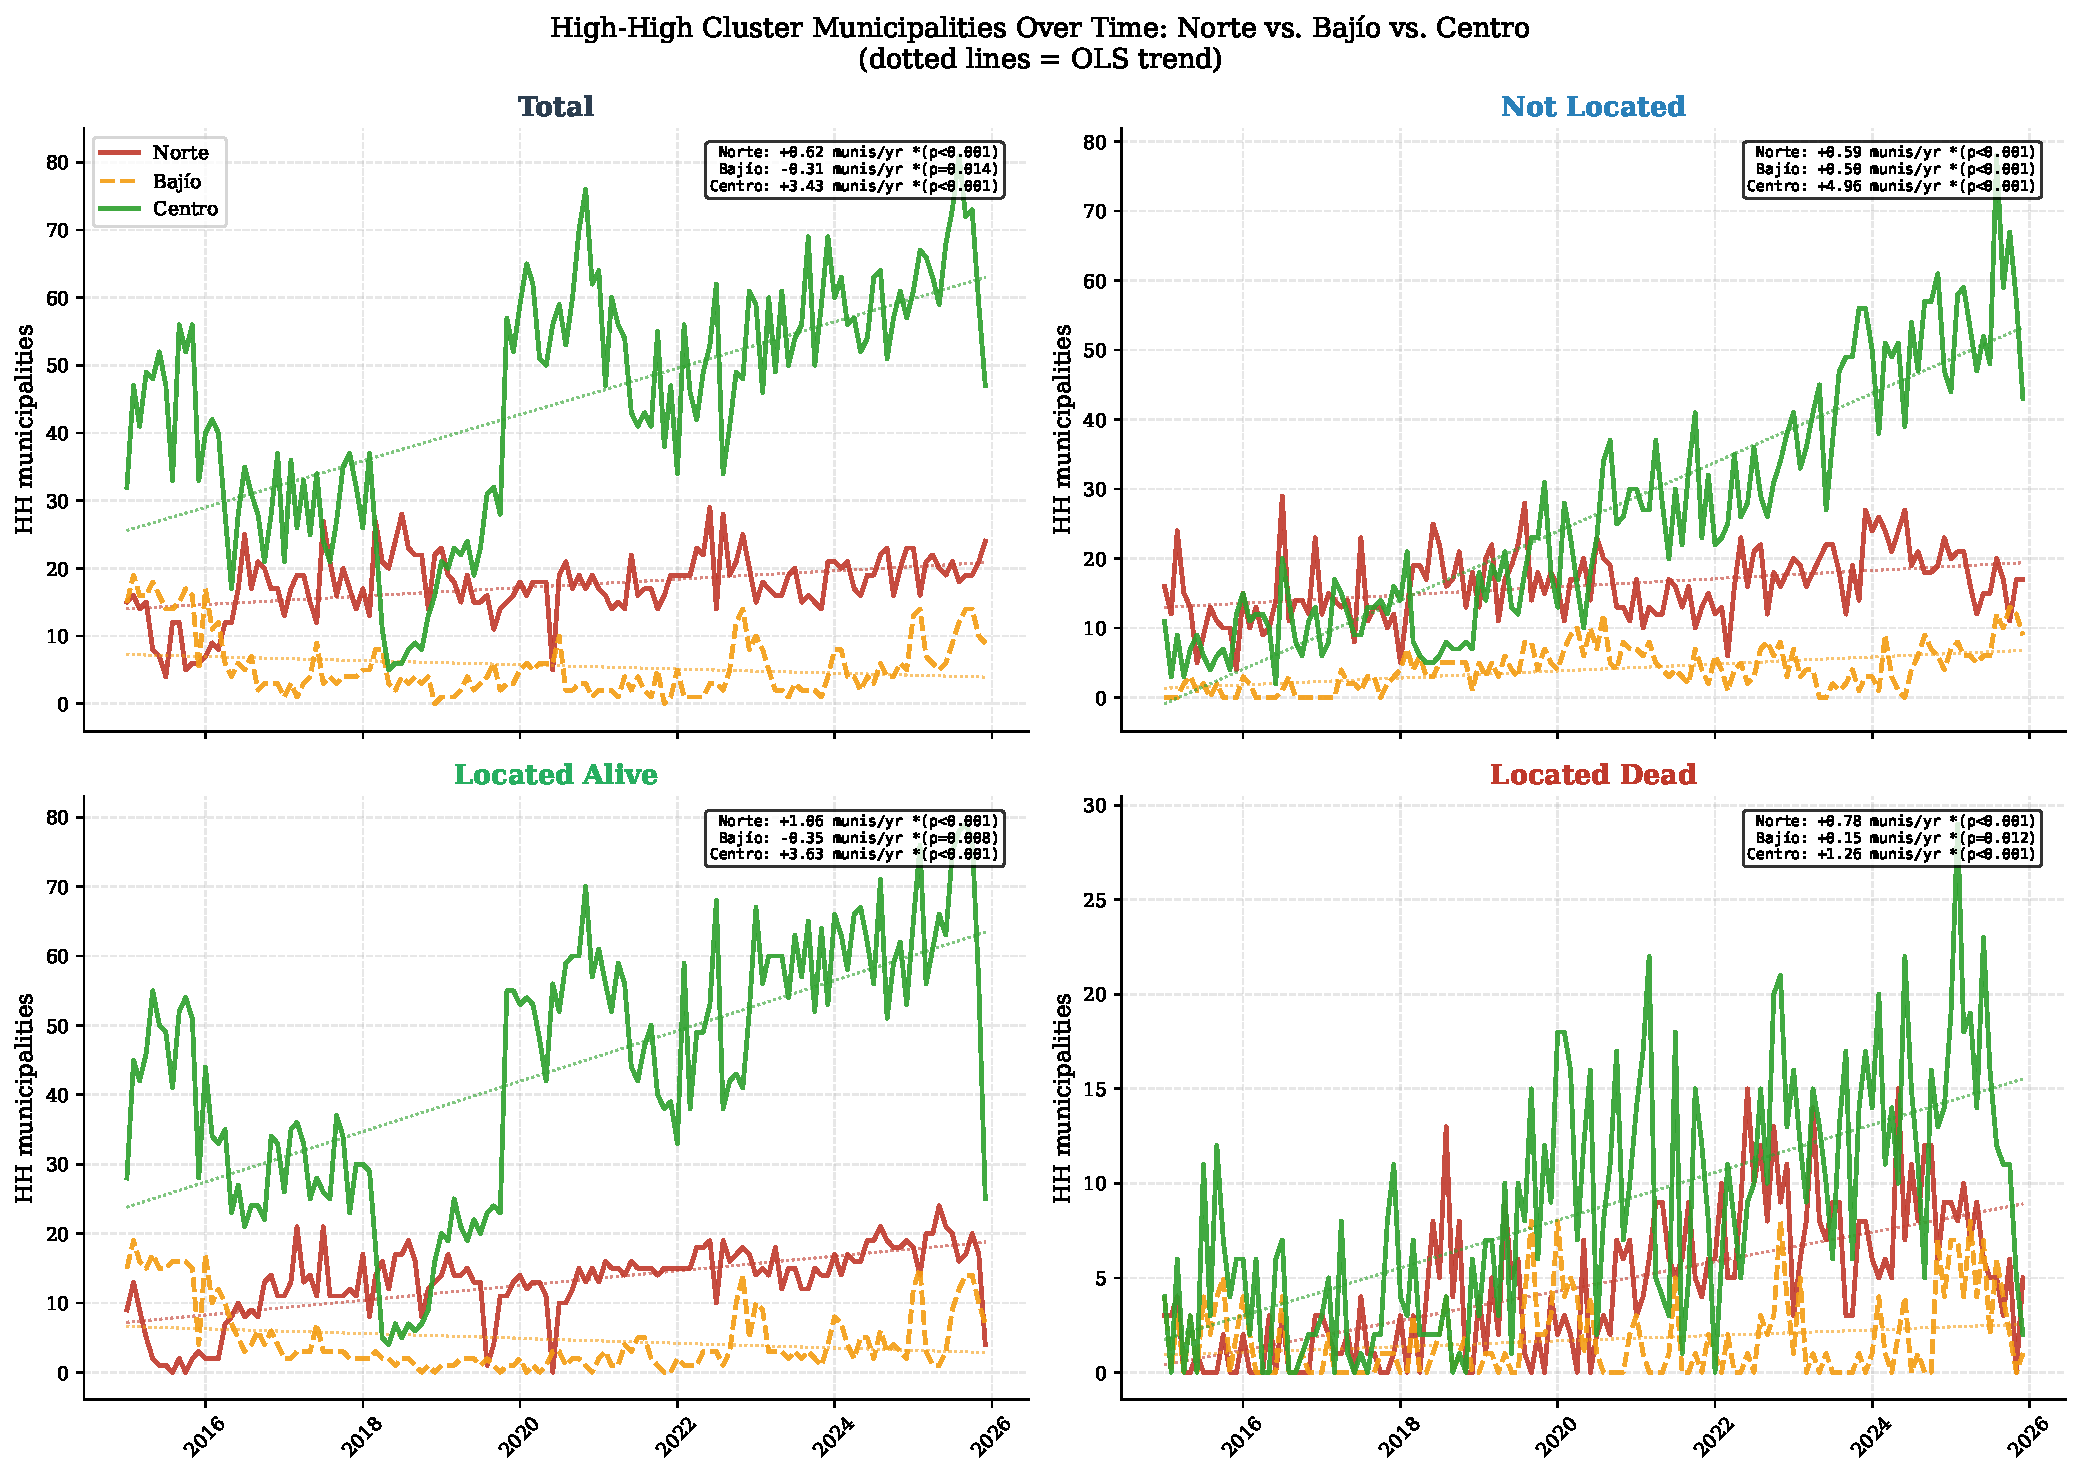
\includegraphics[width=\textwidth]{figures/fig5_hh_trend_norte_bajio.pdf}
  \caption{Monthly count of HH cluster municipalities in Norte (blue), Baj\'{i}o (orange), and Centro (green) by outcome status, \studyperiod{}.
           Dashed lines indicate OLS trends.
           Slopes (municipalities/year) annotated with Newey-West significance.}
  \label{fig:hh_trend}
\end{figure}

\subsubsection{The Norte Consolidation}

Norte shows consistent positive growth in HH municipalities across all four statuses: Total $+0.62^{*}$, Not Located $+0.59^{**}$, Located Alive $+1.06^{***}$, and Located Dead $+0.78^{***}$.
This multi-status consolidation suggests an entrenched organized crime presence---people are going missing, being found alive, \emph{and} being found dead at increasing rates in the same region.
The simultaneous growth of Located Alive and Located Dead hotspots in Norte may reflect a combination of high disappearance incidence and relatively developed forensic and search infrastructure: bodies and living persons are recovered because institutional capacity exists to register them, even as the underlying crisis deepens.

\subsubsection{The Baj\'{i}o Hypothesis: Rejected}

The earlier annual pipeline and existing literature \citep{cadena_garrocho_2019} suggested a ``rising Baj\'{i}o'' pattern driven by cartel territorial expansion into the Guanajuato--Jalisco corridor.
The monthly analysis rejects this hypothesis for the aggregate measure: Baj\'{i}o Total slope is $-1.09$ municipalities per year ($p = 0.024$), indicating a \emph{declining} hotspot footprint.
Located Alive in Baj\'{i}o also shows a negative (though non-significant) slope ($-0.47$, $p = 0.410$).
Located Dead trends positive ($+0.22$) but is not statistically significant ($p = 0.317$).
Not Located is similarly non-significant ($+0.24$, $p = 0.531$).

The Baj\'{i}o finding illustrates a broader methodological point: aggregate analyses can mask compositional dynamics that only become visible with outcome disaggregation and monthly resolution.

\subsubsection{Bookend Comparison}

Figure~\ref{fig:lisa_comparison} compares LISA maps for \bookendstart{} and \referencemonth{} for Located Alive and Located Dead, visualizing the geographic shift over the study period.
The expansion of Located Alive HH clusters from a concentrated Norte-Centro nucleus in 2015 to a broader multi-regional pattern by 2025 is clearly visible.
Located Dead clusters remain sparse at both endpoints, though a new cluster in Guanajuato emerges by 2025.

\begin{figure}[htbp]
  \centering
  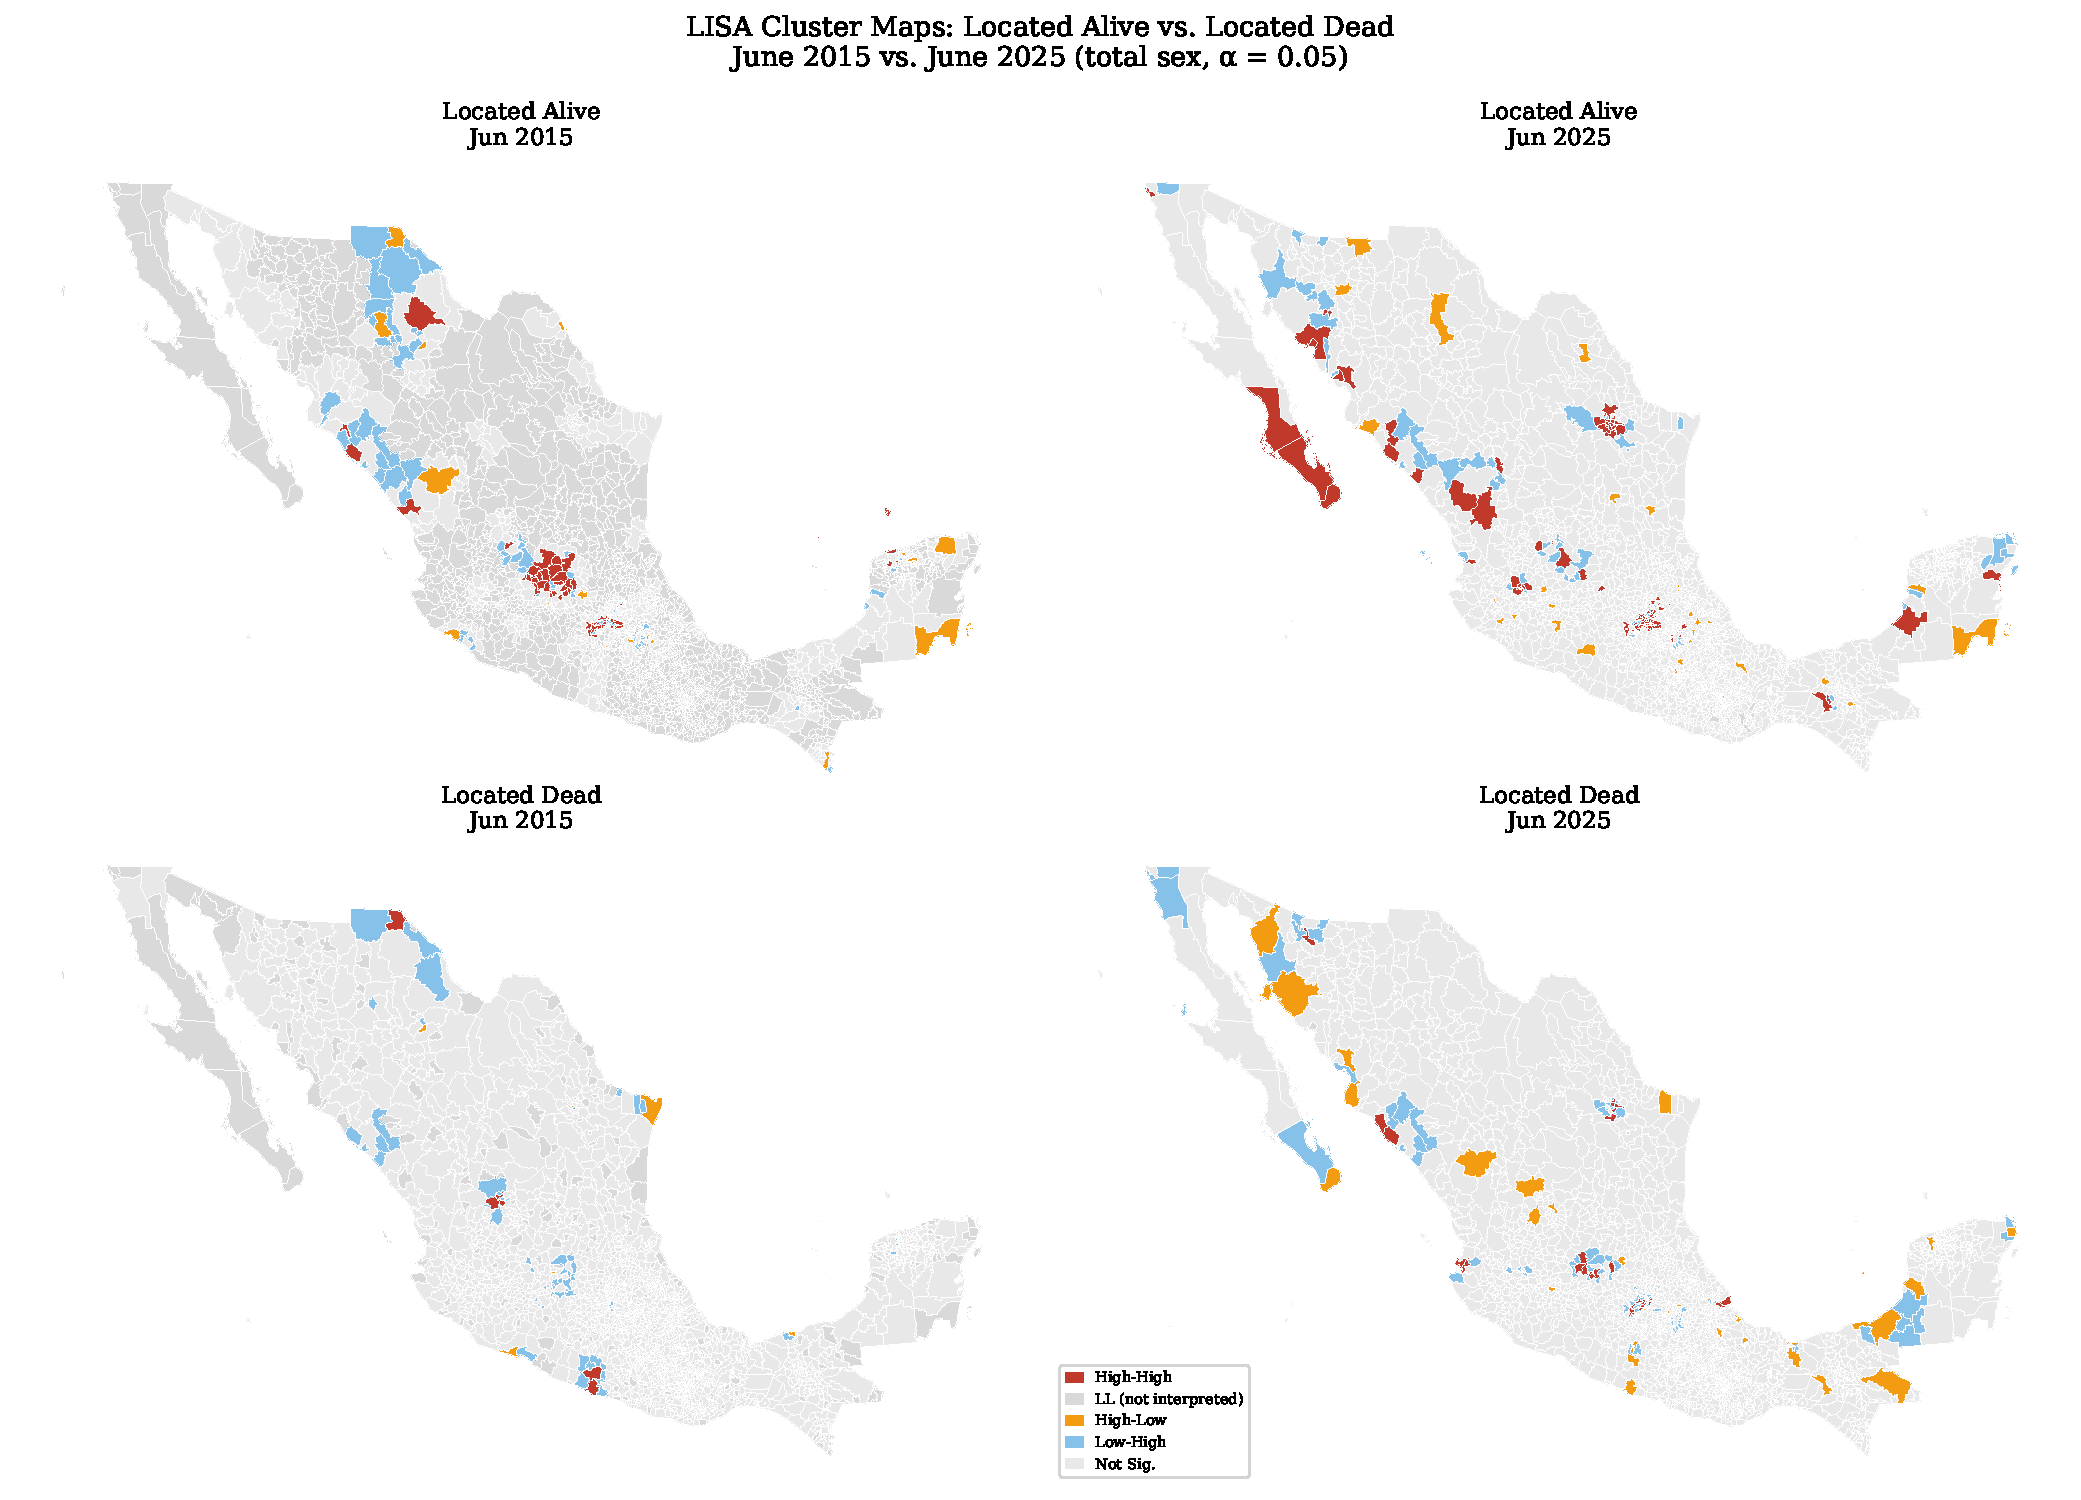
\includegraphics[width=\textwidth]{figures/fig6_lisa_maps_2015_vs_2025.pdf}
  \caption{LISA cluster maps for Located Alive (top) and Located Dead (bottom),
           \bookendstart{} (left) vs.\ \referencemonth{} (right).
           Projection: EPSG:6372.}
  \label{fig:lisa_comparison}
\end{figure}

Figure~\ref{fig:heatmap} provides a synoptic view of regional dynamics through a heatmap of HH municipality counts across 11 June snapshots (2015--2025) for all four statuses.
The chi-square tests for distributional change between \bookendstart{} and \referencemonth{} are significant for all statuses: Total ($\chi^2 = 9.5$, $p = 0.050$), Not Located ($\chi^2 = 16.5$, $p = 0.002$), Located Alive ($\chi^2 = 17.7$, $p = 0.001$), and Located Dead ($\chi^2 = 14.1$, $p = 0.007$).

\begin{figure}[htbp]
  \centering
  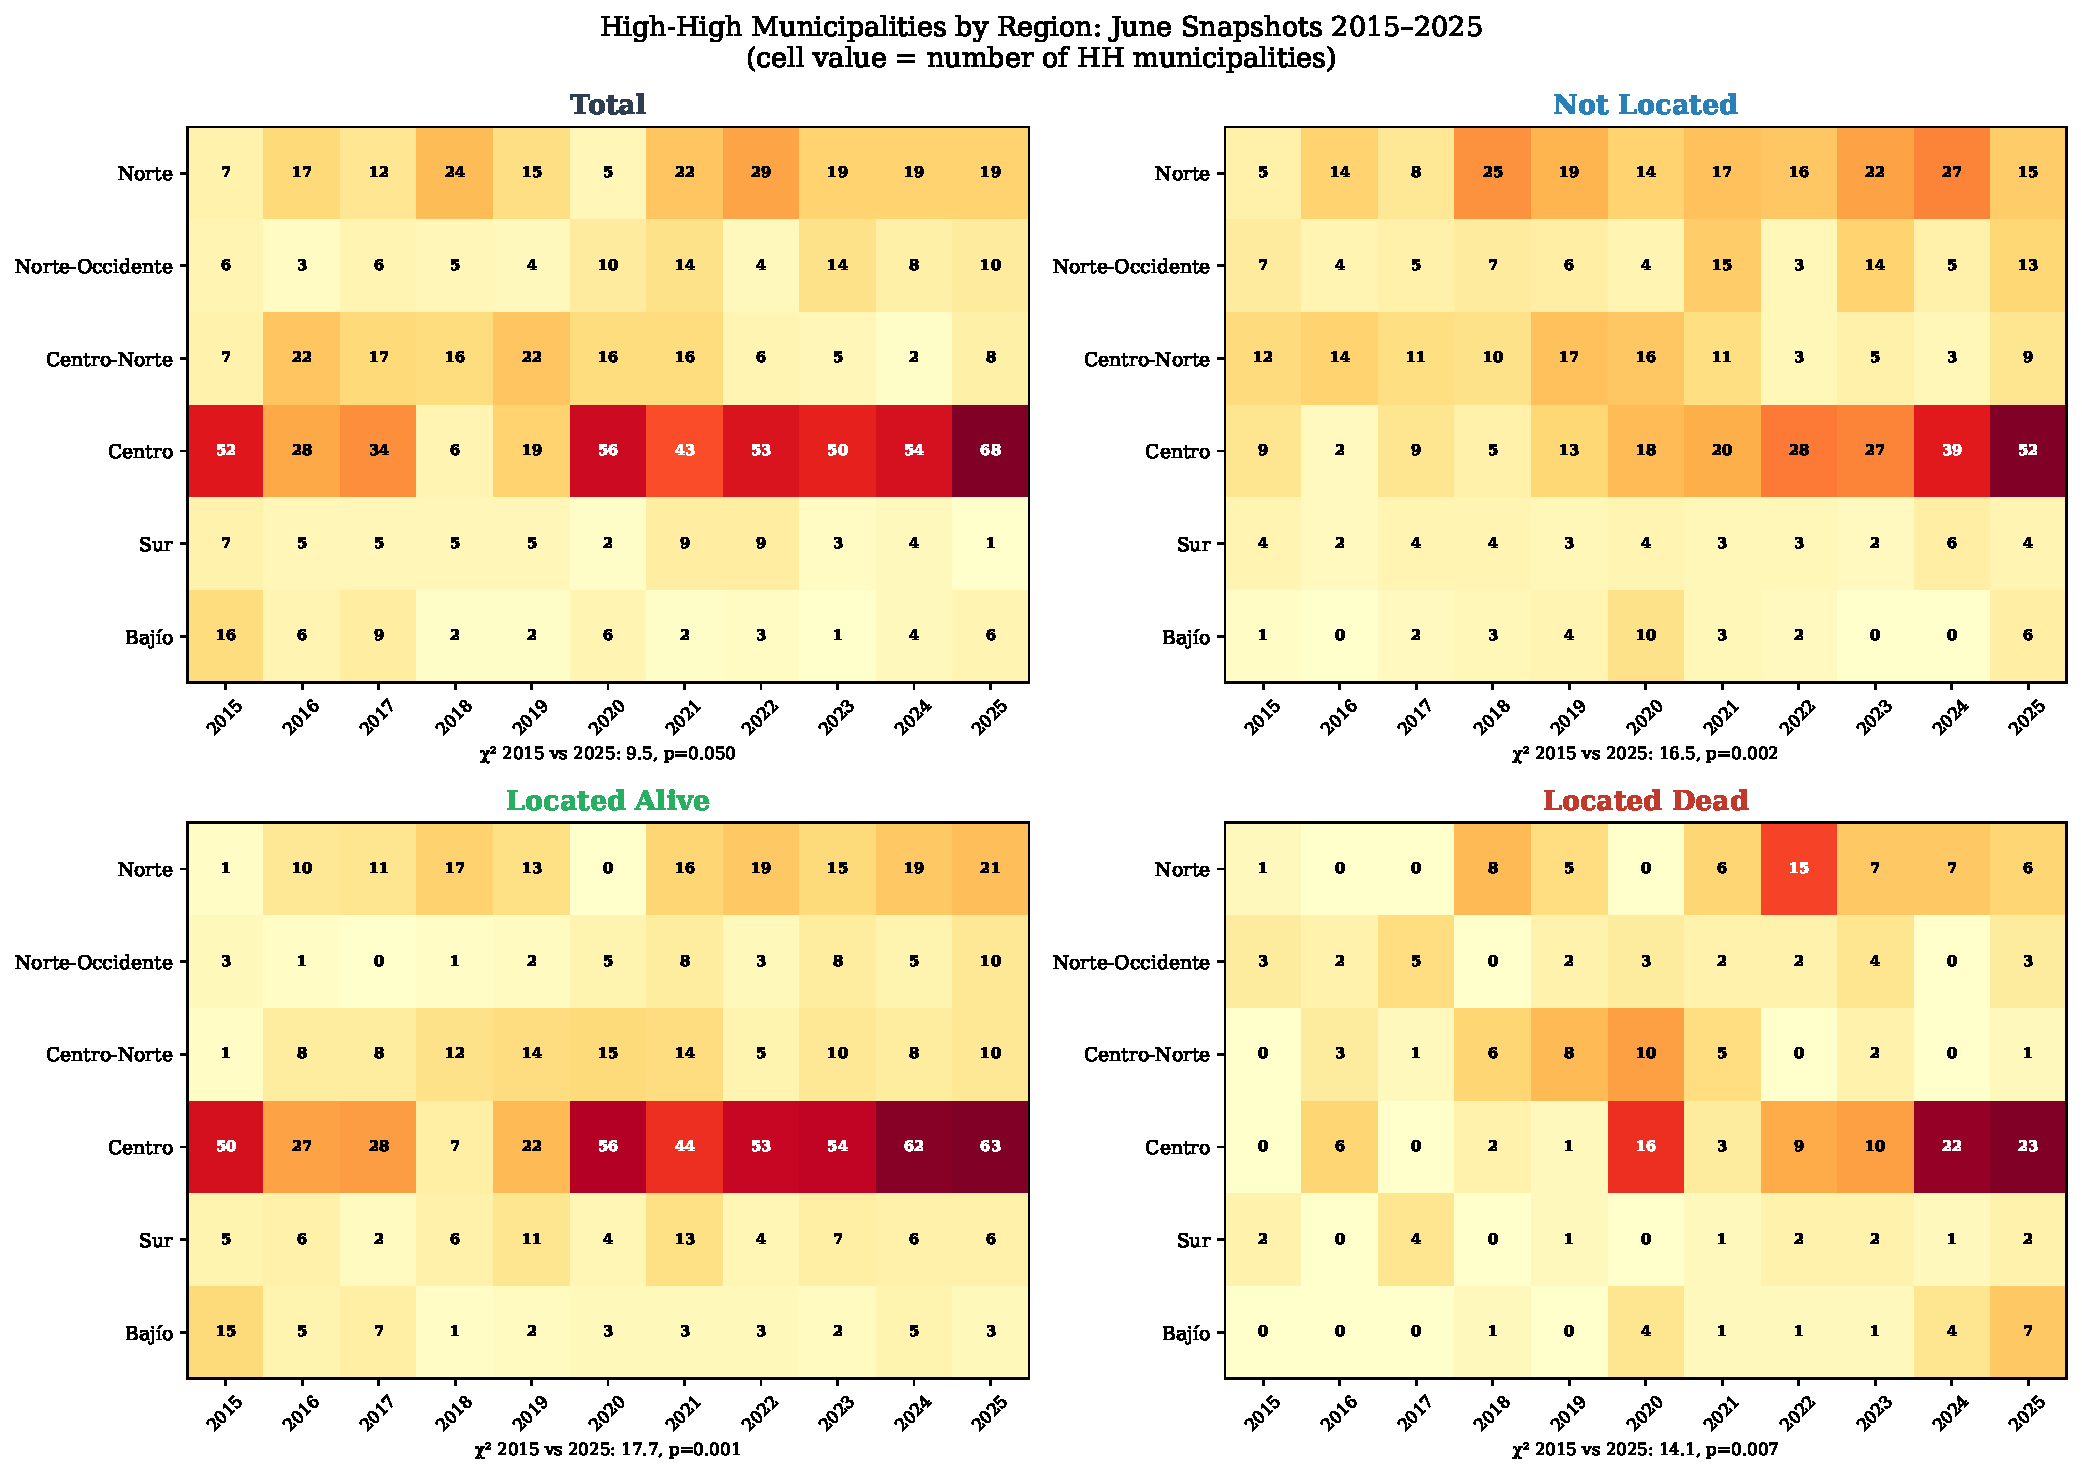
\includegraphics[width=\textwidth]{figures/fig8_regional_hh_heatmap.pdf}
  \caption{Regional HH heatmap: number of HH municipalities by region (rows) and June snapshot year (columns), four panels by outcome status.
           \bookendstart{} vs.\ \referencemonth{}.}
  \label{fig:heatmap}
\end{figure}
